\chapter{Sampling}
\label{ch:sampling}

\section{Poisson Disk Sampling}
\label{sec:poisson_disk_sampling}

\subsection{Overview}
\index{Poisson disk sampling}Poisson disk sampling is a technique for generating a set of points in a multidimensional space such that no two points are closer to each other than a specified minimum distance $r$. The resulting distribution has a ``\index{blue noise}blue noise'' characteristic: the points are tightly packed but avoid the structured look of a grid and the clumping found in pure random (white noise) sampling. This makes it ideal for computer graphics, procedural generation, and sensor placement~\cite{cook1986}.

\subsection{Definitions}
\begin{definition}[Minimum Distance ($r$)]\label{def:minimum_distance}
The radius of an exclusion disk around each point. No two generated points may be closer than $r$ to each other, ensuring a minimum spacing constraint.
\end{definition}

\begin{definition}[Blue Noise]\label{def:blue_noise}
A random distribution where low-frequency components are minimized in the power spectrum, resulting in a visually pleasing and uniform distribution. Formally, the Fourier transform of the point set has negligible energy below a cutoff frequency determined by the density~\cite{cook1986}.
\end{definition}

\begin{definition}[Bridson's Algorithm]\label{def:bridson_algorithm}
A fast $O(n)$ algorithm for generating \index{Poisson disk sampling}Poisson disk samples in any dimension, introduced by Robert Bridson~\cite{bridson2007}. It uses a background grid for $O(1)$ proximity queries and an active list for incremental growth.
\end{definition}

\begin{definition}[Rejection Sampling]\label{def:rejection_sampling}
A naive approach where random points are generated and discarded if they fall within distance $r$ of any existing point. The acceptance rate decreases rapidly as the domain fills, making it $O(n^2)$ in the worst case~\cite{lagae2008}.
\end{definition}

\subsection{Theory}
Bridson's algorithm~\cite{bridson2007} is the standard for efficient Poisson disk sampling:
\begin{enumerate}
    \item \textbf{Initialize}: Place an initial point randomly in the domain and add it to an \textbf{active list}.
    \item \textbf{Grid}: Initialize a background grid with cell size $r / \sqrt{d}$ (where $d$ is dimension) to ensure each cell can contain at most one point. This guarantees that proximity checks only need to examine the 9 (in 2D) or 27 (in 3D) neighboring cells.
    \item \textbf{Active Sampling}: While the active list is not empty:
    \begin{itemize}
        \item Pick a random point $P$ from the active list.
        \item Generate up to $k$ candidates in an annulus $[r, 2r]$ around $P$.
        \item For each candidate $Q$, check if it is within distance $r$ of any existing points (using the grid for $O(1)$ lookups).
        \item If $Q$ is valid, add it to the grid and the active list.
        \item If no candidates are found after $k$ trials, remove $P$ from the active list.
    \end{itemize}
\end{enumerate}

\begin{theorem}[Complexity of Bridson's Algorithm]\label{thm:bridson_complexity}
Bridson's algorithm generates $n$ Poisson disk samples in expected $O(n)$ time and $O(n)$ space, assuming a fixed minimum distance $r$ and dimension $d$.
\end{theorem}

\begin{proof}
Each of the $n$ points is processed at most once from the active list. For each active point, at most $k$ candidates are generated, and each candidate requires $O(1)$ time for the grid-based neighborhood query (since at most $3^d$ cells need to be checked). When a candidate is accepted, the grid insertion is $O(1)$. A point is removed from the active list after $k$ failed trials, so the total number of candidate tests is at most $kn = O(n)$. The grid stores at most $O(n)$ points in $O(n)$ cells. Thus the total expected time is $O(n)$ and space is $O(n)$~\cite{bridson2007}.
\end{proof}

\begin{figure}[htbp]
\centering
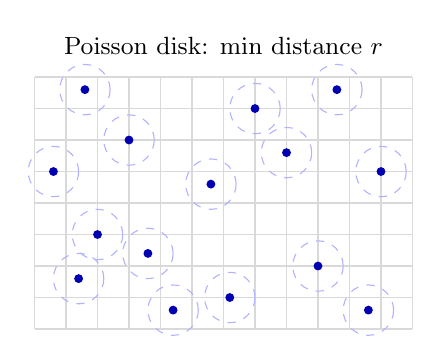
\begin{tikzpicture}[scale=0.8]
  \draw[gray!30,thin] (0,0) grid[step=0.5] (6,4);
  \foreach \x/\y in {0.7/0.8, 1.8/1.2, 3.1/0.5, 4.5/1.0, 5.3/0.3, 0.3/2.5, 1.5/3.0, 2.8/2.3, 4.0/2.8, 5.5/2.5, 1.0/1.5, 3.5/3.5, 4.8/3.8, 2.2/0.3, 0.8/3.8} {
    \fill[blue!70!black] (\x,\y) circle (2pt);
    \draw[blue!30,thin,dashed] (\x,\y) circle (0.4);
  }
  \node[font=\small] at (3,4.5) {Poisson disk: min distance $r$};
\end{tikzpicture}
\caption{Poisson disk sampling: points are placed with minimum distance $r$ between any pair.}
\label{fig:poisson_disk}
\end{figure}


\begin{example}[Poisson Disk Sampling Trace on a $4 \times 4$ Grid]\label{ex:poisson_disk_trace}
Consider a small domain $[0, 4] \times [0, 4]$ with $r = 1.5$ and $k = 8$.
\begin{enumerate}
    \item Seed: Place $P_1 = (2.0, 2.0)$. Grid cell size $= 1.5/\sqrt{2} \approx 1.06$, so the grid is $4 \times 4$.
    \item Active list: $[P_1]$. Pick $P_1$, generate candidates around it. Suppose $Q_1 = (0.8, 1.2)$ passes the distance check ($|P_1 Q_1| \approx 1.44 < 1.5$---rejected). Try again: $Q_2 = (3.3, 1.1)$, distance $\approx 1.35 < 1.5$---rejected. After 8 failures, remove $P_1$ from active list.
    \item Since only one point was placed and no new points accepted, the result is $\{(2.0, 2.0)\}$.
\end{enumerate}
For a larger domain with more seed attempts, the algorithm fills the space more densely, with each new point guaranteed to be at least $r$ from all others.
\end{example}

\subsection{Pseudocode}
\begin{algorithm}
\caption{Poisson Disk Sampling}\label{alg:poisson_disk_sampling}
\begin{algorithmic}
\Function{PoissonDiskSampling}{width, height, r, k=30}
    \Comment{1. Initialize Grid}
    \State $cell\_size \gets r / \sqrt{2}$
    \State $cols \gets \lceil width / cell\_size \rceil$
    \State $rows \gets \lceil height / cell\_size \rceil$
    \State $grid \gets \text{array}[cols][rows] \text{ initialized to None}$

    \Comment{2. Seed Point}
    \State $start\_p \gets \text{Point}(\text{random}(width), \text{random}(height))$
    \State $active\_list \gets [start\_p]$
    \State $\text{InsertIntoGrid}(start\_p, grid, cell\_size)$
    \State $points \gets [start\_p]$

    \Comment{3. Main Loop}
    \While{$active\_list$ is not empty}
        \State $p \gets \text{random.choice}(active\_list)$
        \State $found \gets \text{False}$

        \For{$\_ \text{ in range}(k)$}
            \Comment{Generate candidate in annulus $[r, 2r]$}
            \State $q \gets \text{GenerateRandomInAnnulus}(p, r, 2 \cdot r)$

            \If{$\text{IsInBounds}(q, width, height)$ \textbf{and} $\text{IsValid}(q, grid, r, cell\_size)$}
                \State $points.\text{append}(q)$
                \State $active\_list.\text{append}(q)$
                \State $\text{InsertIntoGrid}(q, grid, cell\_size)$
                \State $found \gets \text{True}$
                \State \textbf{break}
            \EndIf
        \EndFor

        \If{$\neg found$}
            \State $active\_list.\text{remove}(p)$
        \EndIf
    \EndWhile

    \Return $points$
\EndFunction
\end{algorithmic}
\end{algorithm}

\subsection{Parameter Selection}
\begin{itemize}
    \item \textbf{Radius ($r$)}: Determines the density of the points.
    \item \textbf{Trials ($k$)}: Typically set to 30. Higher $k$ results in tighter packing but increases computation time.
    \item \textbf{Variable Radius}: The algorithm can be adapted to use a varying $r(x, y)$ based on an importance map or image brightness.
\end{itemize}

\subsection{Complexity}
\begin{itemize}
    \item \textbf{Time Complexity}: $O(n)$ where $n$ is the number of points generated, thanks to the grid-based spatial lookup (\cref{thm:bridson_complexity}).
    \item \textbf{Space Complexity}: $O(n)$ to store the points and the grid.
\end{itemize}

\subsection{Usages}
\begin{itemize}
    \item \textbf{Computer Graphics}: Placing objects (like trees or grass) in a natural-looking distribution.
    \item \textbf{Rendering}: Anti-aliasing and jittered sampling for ray tracing.
    \item \textbf{Image Processing}: Halftoning and stippling (representing an image with dots).
    \item \textbf{Procedural Content Generation}: Generating city layouts or dungeon rooms.
    \item \textbf{Physical Simulation}: Initializing particles for fluid or granular simulations.
\end{itemize}

\subsection{Testing Methods and Edge Cases}
\begin{itemize}
    \item \textbf{Distance Constraint}: Verify that for all pairs $(P_i, P_j)$, $dist(P_i, P_j) \ge r$.
    \item \textbf{Boundary Handling}: Ensure points are correctly generated near the edges of the domain.
    \item \textbf{Clumping}: Check the Fourier transform of the point set to verify the blue noise profile (lack of low-frequency spikes).
    \item \textbf{Empty Result}: If the domain is smaller than $r$, the algorithm should return at most one point.
    \item \textbf{Grid Overflow}: Ensure the grid coordinates are correctly clamped to the array bounds.
\end{itemize}

\subsection{References}
\begin{itemize}
    \item Bridson, R. (2007). ``Fast Poisson disk sampling in arbitrary dimensions''. SIGGRAPH Sketches.
    \item Cook, R. L. (1986). ``Stochastic sampling in computer graphics''. ACM Transactions on Graphics.
    \item Lagae, A., \& Dutr\'{e}, P. (2008). ``A comparison of methods for generating Poisson disk distributions''. Computer Graphics Forum.
    \item Wikipedia: Poisson disk sampling
\end{itemize}


\section{Halton Points}
\label{sec:halton_points}

\subsection{Overview}
\index{Halton sequence}Halton sequences are a type of \index{low-discrepancy sequence}low-discrepancy sequence used to generate points in a $d$-dimensional space. Unlike pseudo-random numbers, which can clump together, low-discrepancy sequences are designed to be ``more uniform than random,'' ensuring that every part of the domain is sampled evenly~\cite{halton1960}. Halton points are a generalization of the 1D \index{van der Corput sequence}van der Corput sequence~\cite{vandercorput1935} to higher dimensions using different prime numbers as bases.

\subsection{Definitions}
\begin{definition}[Low-Discrepancy Sequence]\label{def:low_discrepancy_sequence}
A sequence of points $\{x_i\}_{i=1}^N$ in $[0,1)^d$ where the \index{discrepancy}discrepancy $D_N$ (a measure of non-uniformity) satisfies $D_N = O(N^{-1} (\log N)^d)$. This is near-optimal by the Schmidt theorem bound, and achieves faster convergence than pseudo-random sequences in \index{quasi-Monte Carlo}Quasi-Monte Carlo integration~\cite{niederreiter1992}.
\end{definition}

\begin{definition}[Quasi-Monte Carlo (QMC)]\label{def:quasi_monte_carlo}
Integration and simulation methods that use low-discrepancy sequences instead of random numbers. QMC achieves a convergence rate of $O(N^{-1})$ for integrands of bounded variation, compared to $O(N^{-1/2})$ for standard Monte Carlo~\cite{halton1960}.
\end{definition}

\begin{definition}[Van der Corput Sequence]\label{def:van_der_corput_sequence}
A 1D sequence in base $b$ formed by reversing the digits of the base-$b$ representation of integers. The $n$-th element is $\phi_b(n) = \sum_{k=0}^{\infty} a_k b^{-(k+1)}$ where $n = \sum_{k=0}^{\infty} a_k b^k$ is the base-$b$ expansion of $n$~\cite{vandercorput1935}.
\end{definition}

\begin{definition}[Discrepancy]\label{def:discrepancy}
A mathematical measure of how ``non-uniform'' a set of points is. For a point set $P = \{x_1, \ldots, x_N\}$ in $[0,1)^d$, the star discrepancy is:
\[
D_N^* = \sup_{\mathbf{b} \in [0,1]^d} \left| \frac{|P \cap [0, \mathbf{b})|}{N} - \text{Vol}([0, \mathbf{b})) \right|.
\]
\end{definition}

\subsection{Theory}
The Halton sequence in $d$ dimensions is constructed by using the first $d$ prime numbers as bases ($p_1, p_2, \dots, p_d$). The $i$-th point in the sequence is:
$$x_i = (\phi_{p_1}(i), \phi_{p_2}(i), \dots, \phi_{p_d}(i))$$
where $\phi_b(i)$ is the \textbf{radical inverse function} in base $b$.

To compute $\phi_b(i)$:
\begin{enumerate}
    \item Write $i$ in base $b$: $i = \sum a_k b^k$.
    \item Reverse the digits and place them after a decimal point: $\phi_b(i) = \sum a_k b^{-(k+1)}$.
\end{enumerate}

Because the prime bases are co-prime, the coordinates in different dimensions are effectively ``de-correlated,'' filling the $d$-dimensional unit hypercube uniformly.

\begin{theorem}[Discrepancy Bound for Halton Sequences]\label{thm:halton_discrepancy}
For the first $N$ points of the $d$-dimensional Halton sequence, the star discrepancy satisfies:
\[
D_N^* = O\!\left(\frac{1}{N} \prod_{i=1}^{d} \log p_i \cdot \log N\right) = O\!\left(\frac{(\log N)^{d+1}}{N}\right).
\]
This is significantly better than the $O(N^{-1/2})$ convergence of pseudo-random Monte Carlo~\cite{halton1960,niederreiter1992}.
\end{theorem}

\begin{proof}
The proof proceeds by the Koksma--Hlawka inequality, which bounds the integration error by the product of the discrepancy $D_N^*$ and the variation of the integrand. For the Halton sequence, the discrepancy is bounded using the Erd\"{o}s--Tur\'{a} inequality on the digital sequence construction. Each coordinate $\phi_{p_i}$ is a van der Corput sequence in base $p_i$, with discrepancy $O(\log p_i / N)$. By the product property of digital sequences~\cite{niederreiter1992}, the multi-dimensional discrepancy is the product of the one-dimensional discrepancies, giving the stated bound.
\end{proof}

\begin{example}[First Five Halton Points in 2D]\label{ex:halton_2d}
Using bases $p_1 = 2$ and $p_2 = 3$:

\begin{center}
\begin{tabular}{cccc}
\toprule
$n$ & $\phi_2(n)$ & $\phi_3(n)$ & $(x, y)$ \\
\midrule
1 & $0.1_2 = 0.5$ & $0.1_3 = 0.\overline{3}$ & $(0.500, 0.333)$ \\
2 & $0.01_2 = 0.25$ & $0.2_3 = 0.\overline{6}$ & $(0.250, 0.667)$ \\
3 & $0.11_2 = 0.75$ & $0.01_3 = 0.1\overline{1}$ & $(0.750, 0.111)$ \\
4 & $0.001_2 = 0.125$ & $0.12_3 = 0.4\overline{4}$ & $(0.125, 0.444)$ \\
5 & $0.101_2 = 0.625$ & $0.22_3 = 0.\overline{7}$ & $(0.625, 0.778)$ \\
\bottomrule
\end{tabular}
\end{center}
Notice how the points are evenly spread across the unit square with no clumping, unlike pseudo-random sampling.
\end{example}

\subsection{Pseudocode}
\begin{algorithm}
\caption{Halton Sequence Generator}\label{alg:halton_sequence}
\begin{algorithmic}
\Function{HaltonSequence}{num\_points, dimensions}
    \State $primes \gets \text{GetFirstPrimes}(dimensions)$
    \State $points \gets []$

    \For{$i \text{ in range}(1, num\_points + 1)$}
        \State $point \gets []$
        \For{$d \text{ in range}(dimensions)$}
            \State $point.\text{append}(\text{RadicalInverse}(i, primes[d]))$
        \EndFor
        \State $points.\text{append}(point)$
    \EndFor

    \Return $points$
\EndFunction

\Statex

\Function{RadicalInverse}{n, base}
    \State $val \gets 0$
    \State $inv\_base \gets 1.0 / base$
    \State $f \gets inv\_base$
    \While{$n > 0$}
        \State $val \gets val + (n \bmod base) \cdot f$
        \State $n \gets \lfloor n / base \rfloor$
        \State $f \gets f \cdot inv\_base$
    \EndWhile
    \Return $val$
\EndFunction
\end{algorithmic}
\end{algorithm}

\subsection{Parameter Selection}
\begin{itemize}
    \item \textbf{Prime Bases}: Must use unique prime numbers for each dimension. Using non-primes or identical bases will lead to strong correlations (linear patterns).
    \item \textbf{Burn-in (Leaping)}: For higher dimensions, the first few hundred points can show patterns. ``Scrambled Halton'' or skipping the initial points can improve uniformity~\cite{niederreiter1992}.
\end{itemize}

\subsection{Complexity}
\begin{itemize}
    \item \textbf{Time Complexity}: $O(N \cdot D \cdot \log_b N)$ to generate $N$ points in $D$ dimensions. Since $b$ is small, this is very fast.
    \item \textbf{Space Complexity}: $O(D)$ to store the current point (or $O(N \cdot D)$ to store the full sequence).
\end{itemize}

\subsection{Usages}
\begin{itemize}
    \item \textbf{Quasi-Monte Carlo Integration}: Estimating high-dimensional integrals with faster convergence ($O(1/N)$) than standard Monte Carlo ($O(1/\sqrt{N})$).
    \item \textbf{Computer Graphics}: Sampling light sources and pixels for ray tracing and path tracing.
    \item \textbf{Physics Simulation}: Initializing particles in a way that minimizes clumping.
    \item \textbf{Global Optimization}: Sampling the search space for black-box optimization algorithms.
    \item \textbf{Financial Modeling}: Pricing complex derivatives where high-dimensional integrals are involved.
\end{itemize}

\subsection{Testing Methods and Edge Cases}
\begin{itemize}
    \item \textbf{Range Check}: All coordinates must be in the interval $[0, 1)$.
    \item \textbf{Uniformity}: Test using the ``Chi-Squared'' test or by calculating the actual discrepancy of the set.
    \item \textbf{Dimension Correlation}: Plot 2D projections of high-dimensional sequences (e.g., dim 10 vs dim 11) to check for ``ghosting'' patterns.
    \item \textbf{Large $N$}: Ensure the radical inverse function doesn't lose precision for very large indices.
    \item \textbf{Base Selection}: Verify that using the same base for two dimensions results in points lying on a single line.
\end{itemize}

\subsection{References}
\begin{itemize}
    \item Halton, J. H. (1960). ``On the efficiency of certain quasi-random sequences of points in evaluating multi-dimensional integrals''. Numerische Mathematik.
    \item Niederreiter, H. (1992). ``Random Number Generation and Quasi-Monte Carlo Methods''. SIAM.
    \item Van der Corput, J. G. (1935). ``Verteilungsfunktionen''. Proc. Akad. Wet. Amsterdam.
    \item Wikipedia: Halton sequence
\end{itemize}


\section{Uniform Random Point Generation}
\label{sec:uniform_random_points}

\subsection{Overview}
\index{uniform random sampling}Generating points uniformly at random inside a
basic shape---square, rectangle, circle, or sphere---is a building block for
Monte Carlo simulation, rendering, and randomized algorithms. Two families of
methods are standard: \textbf{rejection sampling}, which works for any shape,
and exact \textbf{transform} methods that map uniform variables onto the shape
without waste~\cite{devroye1986}. For the square and rectangle the task is
trivial (independent coordinates); for the circle and sphere a naive
coordinate-based approach is biased, so the Jacobian of the mapping must be
corrected.

\subsection{Definitions}
\begin{definition}[Uniform Point Set]\label{def:uniform_point_set}
A point set is \emph{uniform} in a region $\Omega \subseteq \mathbb{R}^d$ if
the number of points in every measurable subset $A \subseteq \Omega$ is
proportional to $\operatorname{Vol}(A)$. Equivalently, the points are drawn
from the uniform measure on $\Omega$.
\end{definition}

\begin{definition}[Rejection Sampling]\label{def:rejection_shape}
\index{rejection sampling}To sample uniformly in a bounded region $\Omega$,
sample candidate points uniformly in a bounding box $B \supseteq \Omega$ and
\emph{accept} those that lie inside $\Omega$. The acceptance rate is
$\operatorname{Vol}(\Omega) / \operatorname{Vol}(B)$.
\end{definition}

\subsection{Theory}
For the axis-aligned rectangle $[x_1, x_2] \times [y_1, y_2]$, two independent
uniform coordinates $u, v \sim \operatorname{Unif}[0, 1)$ give the exact uniform point
$(x_1 + u \Delta x, \, y_1 + v \Delta y)$.

For the disk of radius $R$, uniform coordinates in $[0, 1)^2$ must be
transformed with the radial density of a disk: radii cluster near the center
if drawn uniformly, so the inverse of the cumulative radial measure is used.

\begin{theorem}[Uniform Disk and Sphere Sampling]\label{thm:uniform_ball}
Let $u, v, w \sim \operatorname{Unif}[0, 1)$ be independent. Then
\begin{itemize}
\item $(\sqrt{u} R \cos 2\pi v, \; \sqrt{u} R \sin 2\pi v)$ is uniform in the
  disk of radius $R$;
\item $u^{1/3} R$ times a unit direction (drawn by Marsaglia's method below)
  is uniform in the ball of radius $R$;
\item $(2x\sqrt{1 - x^2 - y^2}, \; 2y\sqrt{1 - x^2 - y^2}, \; 1 - 2(x^2 + y^2))$
  for $(x, y)$ uniform in the unit disk is uniform on the unit
  sphere~\cite{marsaglia1972}.
\end{itemize}
\end{theorem}
\begin{proof}[Proof sketch]
The first claim follows from the Jacobian of the polar map: the density of a
disk is uniform in the area element $r\,dr\,d\theta$, so the radius must be
distributed as $\sqrt{u}$. The last claim is Marsaglia's method: a uniform
point in the unit disk, lifted to the sphere by the inverse stereographic
mapping scaled by $r \mapsto (2\sqrt{1-r^2}, 1 - 2r^2)$, preserves the uniform
area measure~\cite{marsaglia1972}.
\end{proof}

Rejection sampling's acceptance rate is the volume ratio: $\pi/4 \approx 0.785$
for a disk in its bounding square, $\pi/6 \approx 0.524$ for a ball in its
bounding cube. The expected number of trials to accept $n$ points is
$n / \text{rate}$.

For the \emph{boundary} of a polygon the uniform measure is arc length, not
area. A point sampled uniformly on the boundary is obtained by choosing an
edge with probability proportional to its length and then sampling uniformly
along that edge; equivalently, invert a uniform variate on the cumulative
perimeter length (arc-length parametrization). For the rectangle
$[x_1, x_2] \times [y_1, y_2]$ with width $w = x_2 - x_1$ and height
$h = y_2 - y_1$, the edge probabilities are
$w, h, w, h$ over the total perimeter $2(w + h)$, so longer sides receive
proportionally more points and no corner or side is over- or
under-sampled.

\subsection{Pseudocode}

\begin{algorithm}
\caption{Uniform Random Points in Basic Shapes}\label{alg:uniform_points}
\begin{algorithmic}
\Function{UniformInRectangle}{x1, x2, y1, y2, n}
    \State \Return $[(x_1 + u \cdot (x_2 - x_1), y_1 + v \cdot (y_2 - y_1)) \text{ for } (u, v) \text{ in }\text{Rand2D}(n)]$
\EndFunction

\Statex

\Function{UniformInCircle}{cx, cy, R, n}
    \State \Return $\big[(cx + \sqrt{u} R \cos 2\pi v,\; cy + \sqrt{u} R \sin 2\pi v) \text{ for } (u, v) \text{ in }\text{Rand2D}(n)\big]$
\EndFunction

\Statex

\Function{UniformOnSphere}{n}
    \State $pts \gets []$
    \While{$|pts| < n$}
        \State $x \gets \operatorname{Unif}[-1, 1]$, \quad $y \gets \operatorname{Unif}[-1, 1]$
        \If{$x^2 + y^2 < 1$} \Comment{reject points outside the unit disk}
            \State $s \gets \sqrt{1 - x^2 - y^2}$
            \State $pts.\text{append}\big((2xs,\; 2ys,\; 1 - 2(x^2 + y^2))\big)$
        \EndIf
    \EndWhile
    \State \Return $pts$
\EndFunction

\Statex

\Function{UniformOnRectangleBoundary}{x1, x2, y1, y2, n}
    \State $w \gets x_2 - x_1$, \quad $h \gets y_2 - y_1$
    \State $perim \gets 2 \cdot (w + h)$
    \State $pts \gets []$
    \For{$i \text{ in range}(n)$}
        \State $s \gets \operatorname{Unif}[0, perim)$ \Comment{arc length along the boundary}
        \If{$s < w$}
            \State $p \gets (x_1 + s, y_1)$
        \ElsIf{$s < w + h$}
            \State $p \gets (x_2, y_1 + (s - w))$
        \ElsIf{$s < 2w + h$}
            \State $p \gets (x_2 - (s - w - h), y_2)$
        \Else
            \State $p \gets (x_1, y_2 - (s - 2w - h))$
        \EndIf
        \State $pts.\text{append}(p)$
    \EndFor
    \State \Return $pts$
\EndFunction

\Statex

\Function{UniformOnPolygonBoundary}{polygon, n}
    \State $L \gets \text{edge lengths of } polygon$ \Comment{edges in CCW order}
    \State $cum \gets \text{cumulative sums of } L$
    \State $pts \gets []$
    \For{$i \text{ in range}(n)$}
        \State $s \gets \operatorname{Unif}[0, cum[\text{last}])$
        \State $j \gets$ first index with $cum[j] > s$ \Comment{binary search}
        \State $t \gets (s - cum[j-1]) / L[j]$
        \State $p \gets (1 - t) \cdot v_j + t \cdot v_{j+1}$
        \State $pts.\text{append}(p)$
    \EndFor
    \State \Return $pts$
\EndFunction
\end{algorithmic}
\end{algorithm}

\subsection{Parameter Selection}
\begin{itemize}
    \item \textbf{Rejection vs.\ Transform}: use rejection for arbitrary
      shapes (polygons, curved regions); use the exact transforms for
      disk/ball/sphere to avoid waste.
    \item \textbf{Seed}: fix the RNG seed for reproducibility in tests.
\end{itemize}

\subsection{Complexity}
\begin{itemize}
    \item \textbf{Transform Methods}: $O(n)$ time and space; no waste.
    \item \textbf{Rejection Sampling}: expected $O(n / \text{rate})$ time;
      worst-case unbounded, but the geometric distribution bound applies.
    \item \textbf{Boundary Sampling}: $O(n)$ for the rectangle (constant work
      per point); $O(n \log m)$ for a general $m$-gon via binary search on the
      cumulative perimeter lengths.
\end{itemize}

\subsection{Usages}
\begin{itemize}
    \item \textbf{Monte Carlo Integration}: estimating areas and volumes
      (hit-or-miss sampling).
    \item \textbf{Rendering}: sampling light sources and area lights.
    \item \textbf{Initialization}: seeding particle and agent simulations.
    \item \textbf{Randomized Geometry}: point-in-polygon testing and random
      inputs for testing geometric algorithms.
\end{itemize}

\subsection{Testing Methods and Edge Cases}
\begin{itemize}
    \item \textbf{Uniformity}: use a Chi-squared test on a sub-grid of the
      shape, or a 1D marginal (e.g., the $x$-marginal of a disk is uniform).
    \item \textbf{Boundary}: points on the boundary should be rare; include or
      exclude boundary deterministically.
    \item \textbf{Radius Distribution}: verify the disk histogram of $r / R$
      is linear (density of $r$ proportional to $r$).
    \item \textbf{Zero-area / degenerate shapes}: a rectangle with
      $x_1 = x_2$ or $R = 0$ must return the boundary or an empty set
      deterministically.
    \item \textbf{Boundary density}: for a $w \times h$ rectangle, the number
      of points on the two horizontal sides must be in ratio $w : h$ (not
      $1 : 1$); points on the boundary must never fall inside the shape.
\end{itemize}

\subsection{References}
\begin{itemize}
    \item Devroye, L. (1986). ``Non-Uniform Random Variate Generation''.
      Springer.
    \item Marsaglia, G. (1972). ``Choosing a point from the surface of a
      sphere''. The Annals of Mathematical Statistics.
\end{itemize}

\section{Random Line Segment Generation}
\label{sec:random_segments}

\subsection{Overview}
\index{random segment generation}Generating random line segments in 2D or 3D
is used for testing segment intersection and arrangement algorithms, for
simulating sensor and cable networks, and for constructing random
inputs~\cite{deberg2008}. The natural model samples the two endpoints
independently from a uniform distribution over the domain, so that every
segment is equally likely up to the position of its two endpoints. An
alternative model fixes the segment length and samples a random direction,
which is the right model for fibers, cracks, and insect paths.

\subsection{Definitions}
\begin{definition}[Random Segment Model]\label{def:random_segment}
A segment in $\mathbb{R}^d$ is a pair of endpoints $a, b$. In the
\emph{independent-endpoint model}, $a$ and $b$ are drawn independently from a
uniform distribution over the domain $\Omega$. In the \emph{fixed-length}
model, a length $\ell$, a midpoint (or base point), and a uniform direction
determine the segment.
\end{definition}

\subsection{Theory}
The independent-endpoint model is exact: because each endpoint is uniform in
$\Omega$, the pair $(a, b)$ is uniform in $\Omega \times \Omega$. A fixed
length requires a uniform random direction, which in 2D is the angle
$\theta \sim \operatorname{Unif}[0, 2\pi)$ and in 3D a unit vector sampled
uniformly on the sphere. A cheap 3D method picks a point in the unit ball and
normalizes it (rejection of the $z$-axis bias of naive polar coordinates), or
uses Marsaglia's method of Section~\ref{sec:uniform_random_points}.

\begin{theorem}[Uniform Endpoints in a Box]\label{thm:random_segment}
If $a, b$ are independent and uniform in a box $\prod_i [x_i, y_i]$, then the
endpoints and the segment are uniformly distributed over all segments whose
endpoints lie in the box. The marginal density of the segment midpoint is not
uniform: it concentrates near the center, since midpoints arise from many
endpoint pairs.
\end{theorem}

\subsection{Pseudocode}

\begin{algorithm}
\caption{Random Line Segment Generation}\label{alg:random_segments}
\begin{algorithmic}
\Function{RandomSegment2D}{x1, x2, y1, y2, n}
    \State \Return $[\text{RandomSegmentInBox}(x_1, x_2, y_1, y_2) \text{ for } \_ \text{ in range}(n)]$
\EndFunction

\Statex

\Function{RandomSegmentInBox}{x1, x2, y1, y2, n}
    \State $a \gets \text{UniformInRectangle}(x_1, x_2, y_1, y_2, 1)[0]$
    \State $b \gets \text{UniformInRectangle}(x_1, x_2, y_1, y_2, 1)[0]$
    \State \Return $(a, b)$
\EndFunction

\Statex

\Function{RandomFixedLengthSegment2D}{cx, cy, ell, n}
    \State \Return $\big[( (cx, cy), (cx + \ell \cos \theta, cy + \ell \sin \theta) ) \text{ for } \theta \sim \operatorname{Unif}[0, 2\pi) \text{ in range}(n)\big]$
\EndFunction

\Statex

\Function{RandomSegment3D}{x1, x2, y1, y2, z1, z2, n}
    \State $pts \gets []$
    \While{$|pts| < 2n$}
        \State $u, v, w \sim \operatorname{Unif}[0, 1)$
        \State $p \gets (x_1 + u(x_2 - x_1), y_1 + v(y_2 - y_1), z_1 + w(z_2 - z_1))$
        \State $pts.\text{append}(p)$
    \EndWhile
    \State \Return $[(pts[2i], pts[2i+1]) \text{ for } i \text{ in range}(n)]$
\EndFunction
\end{algorithmic}
\end{algorithm}

\subsection{Parameter Selection}
\begin{itemize}
    \item \textbf{Endpoint model vs.\ fixed length}: choose the independent
      endpoint model for intersection and arrangement stress tests; fixed
      length for fiber and crack models.
    \item \textbf{Seed}: fix the RNG seed for reproducible random inputs.
\end{itemize}

\subsection{Complexity}
\begin{itemize}
    \item \textbf{Time}: $O(n)$ to generate $n$ segments.
    \item \textbf{Space}: $O(n)$ to store the segments; $O(1)$ streaming.
\end{itemize}

\subsection{Usages}
\begin{itemize}
    \item \textbf{Testing segment intersection} algorithms with large random
      inputs.
    \item \textbf{Simulating sensor links}, cables, and cracks.
    \item \textbf{Arrangement} experiments and \textbf{sweep-line} stress
      tests.
\end{itemize}

\subsection{Testing Methods and Edge Cases}
\begin{itemize}
    \item \textbf{Endpoint Range}: verify all endpoints lie in the box.
    \item \textbf{Count}: verify exactly $n$ segments are returned.
    \item \textbf{Distinctness}: for the independent model, degenerate
      zero-length segments are possible but should be rare; decide whether to
      keep or reject them.
    \item \textbf{3D Direction}: for fixed length in 3D, verify the direction
      vectors have norm $\ell$ and are isotropically distributed.
\end{itemize}

\subsection{References}
\begin{itemize}
    \item Devroye, L. (1986). ``Non-Uniform Random Variate Generation''.
      Springer.
    \item de Berg, M., Cheong, O., van Kreveld, M., \& Overmars, M. (2008).
      ``Computational Geometry: Algorithms and Applications''. Springer.
\end{itemize}

\section{Random Polygon Generation}
\label{sec:random_polygons}

\subsection{Overview}
\index{random polygon generation}Generating random convex and concave
(simple) polygons in 2D provides stress tests for polygon algorithms:
triangulation, point-in-polygon, convex partitioning, and boolean
operations~\cite{deberg2008}. The two standard constructions are
\textbf{angle-sorted points on a curve} for convex polygons, and
\textbf{angular sorting around a center} for concave polygons. Both run in
$O(n \log n)$ time and are easy to implement correctly.

\subsection{Definitions}
\begin{definition}[Random Convex Polygon]\label{def:random_convex_polygon}
A convex polygon with $n$ vertices sampled by sorting $n$ angles uniformly in
$[0, 2\pi)$ and placing the corresponding points on the unit circle (or an
ellipse/randomly scaled radius).
\end{definition}

\begin{definition}[Random Simple Polygon]\label{def:random_simple_polygon}
A simple (non-self-intersecting) polygon built by ordering points by their
polar angle around their centroid, giving a star-shaped polygon; a further
random radial perturbation can introduce reflex (concave) vertices while
preserving simplicity.
\end{definition}

\subsection{Theory}
Sorting points by polar angle around any point inside their convex hull
produces a simple polygon: the edges of the star-shaped polygon do not cross.
For the convex case, points on a strictly convex curve (a circle or ellipse)
sorted by angle give a convex polygon. The polygon is convex if and only if
every interior angle is less than $\pi$; an $O(n)$ check of the turn direction
at each vertex certifies this.

\begin{theorem}[Star-Shaped Polygonization]\label{thm:star_polygonization}
If $P = \{p_1, \dots, p_n\}$ are in general position and $c$ is a point in
their convex hull, then the polygon obtained by connecting the points sorted
by polar angle around $c$ is simple and star-shaped with kernel containing
$c$~\cite{deberg2008}.
\end{theorem}
\begin{proof}[Proof sketch]
Every edge of the sorted polygon bounds a triangle with apex $c$ that lies
inside the polygon; adjacent triangles meet only along shared edges, so the
polygon is simple and every point is visible from $c$.
\end{proof}

\subsection{Pseudocode}

\begin{algorithm}
\caption{Random Polygon Generation}\label{alg:random_polygons}
\begin{algorithmic}
\Function{RandomConvexPolygon}{n}
    \State $\theta \gets \text{sort}(\operatorname{Unif}[0, 2\pi) \text{ for } \_ \text{ in range}(n))$
    \State $r \gets \operatorname{Unif}[0.5, 1.0) \text{ for } \_ \text{ in range}(n)$
    \State \Return $[(r_i \cos \theta_i, r_i \sin \theta_i) \text{ for } i \text{ in range}(n)]$
\EndFunction

\Statex

\Function{RandomSimplePolygon}{n}
    \State $p \gets \text{RandomConvexPolygon}(n)$
    \State $c \gets \operatorname{mean}(p)$
    \State $q \gets \text{sort}(p, \text{key} = \text{angle around } c)$
    \For{$i \text{ in range}(n)$}
        \If{$\text{reflex vertex at } q_i$} \Comment{flip to concave by radial move}
            \State $q_i \gets c + (1 + \varepsilon_i) \cdot (q_i - c)$
        \EndIf
    \EndFor
    \State \Return $q$
\EndFunction
\end{algorithmic}
\end{algorithm}

\subsection{Parameter Selection}
\begin{itemize}
    \item \textbf{Radius range}: keep $r \in [0.5, 1.0)$ so points stay away
      from the origin and the polygon is not degenerate.
    \item \textbf{Perturbation}: small $\varepsilon_i$ moves in the radial
      direction create reflex vertices without destroying simplicity; large
      moves can cause self-intersection.
\end{itemize}

\subsection{Complexity}
\begin{itemize}
    \item \textbf{Time}: $O(n \log n)$ for sorting the angles; $O(n)$ for the
      perturbation and the convexity check.
    \item \textbf{Space}: $O(n)$.
\end{itemize}

\subsection{Usages}
\begin{itemize}
    \item \textbf{Testing triangulation, point-in-polygon, and boolean
      operations} on large random inputs.
    \item \textbf{Benchmarking} convex partitioning (Keil--Snoeyink) and art
      gallery algorithms on concave polygons.
\end{itemize}

\subsection{Testing Methods and Edge Cases}
\begin{itemize}
    \item \textbf{Simplicity}: verify no two edges intersect (except adjacent
      edges at shared vertices).
    \item \textbf{Convexity}: for the convex generator, check all interior
      angles $< \pi$ (positive turn direction at every vertex).
    \item \textbf{Vertex Count}: the polygon has exactly $n$ distinct
      vertices.
    \item \textbf{Degenerate cases}: reject duplicate angles and points at the
      origin to keep the polygon simple.
\end{itemize}

\subsection{References}
\begin{itemize}
    \item de Berg, M., Cheong, O., van Kreveld, M., \& Overmars, M. (2008).
      ``Computational Geometry: Algorithms and Applications''. Springer.
    \item Devroye, L. (1986). ``Non-Uniform Random Variate Generation''.
      Springer.
\end{itemize}

\section{Random Walk}
\label{sec:random_walk}

\subsection{Overview}
A \index{random walk}random walk is a mathematical object, known as a stochastic or random process, that describes a path consisting of a succession of random steps on some mathematical space such as the integers or a 2D/3D grid. In computational geometry and physics, random walks are used to model \index{Brownian motion}Brownian motion, \index{diffusion}diffusion, and to approximate the solutions of various partial differential equations (PDEs) through \index{Monte Carlo method}Monte Carlo methods~\cite{pearson1905}.

\subsection{Definitions}
\begin{definition}[Step Size ($\ell$)]\label{def:step_size}
The distance moved in a single step of the random walk. This may be fixed or drawn from a distribution (e.g., Gaussian).
\end{definition}

\begin{definition}[Lattice Walk]\label{def:lattice_walk}
A random walk restricted to a discrete grid (e.g., integer coordinates). At each step, the walker moves to one of the neighboring lattice points with prescribed probabilities.
\end{definition}

\begin{definition}[Isotropic Walk]\label{def:isotropic_walk}
A walk where every direction is equally likely. In 2D, the step direction $\theta$ is uniformly distributed on $[0, 2\pi)$.
\end{definition}

\begin{definition}[Mean Squared Displacement (MSD)]\label{def:msd}
A measure of how far the walker deviates from its starting point over time. For a simple $d$-dimensional random walk with step size $\ell$, $\text{MSD}(n) = \langle |\mathbf{r}_n - \mathbf{r}_0|^2 \rangle = d \cdot \ell^2 \cdot n$, so $\text{MSD} \propto t$~\cite{spitzer1976}.
\end{definition}

\subsection{Theory}
The theory of random walks is closely related to the \index{diffusion equation}diffusion equation $\frac{\partial \phi}{\partial t} = D \nabla^2 \phi$~\cite{spitzer1976}.
\begin{enumerate}
    \item \textbf{1D Walk}: A walker starts at 0 and moves +1 or -1 with probability $1/2$. After $n$ steps, the expected position is 0, but the standard deviation is $\sqrt{n}$.
    \item \textbf{2D/3D Walk}: The walker moves in a random direction. \index{Polya's recurrence theorem}Polya's Theorem~\cite{polya1921} states that a random walk on a 2D lattice is ``recurrent'' (it will return to the start with probability 1), while in 3D it is ``transient'' (it may never return).
    \item \textbf{Walk on Meshes}: A random walk on a mesh jumps from a vertex to one of its adjacent vertices. The probability of choosing a neighbor can be uniform ($1/\text{degree}$) or weighted by edge length or cotangent weights to simulate specific geometric properties.
\end{enumerate}

\begin{theorem}[Polya's Recurrence Theorem]\label{thm:polya_recurrence}
A simple random walk on the $\mathbb{Z}^d$ lattice is recurrent (returns to the origin with probability 1) for $d = 1$ and $d = 2$, and transient (returns with probability less than 1) for $d \ge 3$. Specifically, the return probability in $d = 3$ is approximately $0.3405$~\cite{polya1921}.
\end{theorem}

\begin{proof}
The probability of return is related to the Green's function $G(\mathbf{0}) = \sum_{n=0}^{\infty} P_n(\mathbf{0} \to \mathbf{0})$, which is the expected number of visits to the origin. The walk is recurrent if and only if $G(\mathbf{0}) = \infty$. For a $d$-dimensional walk, the return probability at step $2n$ is:
\[
P_{2n}(\mathbf{0} \to \mathbf{0}) \sim \frac{C_d}{n^{d/2}}
\]
for some constant $C_d > 0$. The series $\sum_{n=1}^{\infty} n^{-d/2}$ converges if and only if $d/2 > 1$, i.e., $d > 2$. Therefore, $G(\mathbf{0}) = \infty$ for $d \le 2$ (recurrent) and $G(\mathbf{0}) < \infty$ for $d \ge 3$ (transient)~\cite{spitzer1976}.
\end{proof}

\begin{example}[1D Random Walk: Expected Position After 100 Steps]\label{ex:random_walk_1d}
Consider a 1D random walk starting at position 0, taking steps of $+1$ or $-1$ with equal probability. After $n = 100$ steps:
\begin{itemize}
    \item Expected position: $\mathbb{E}[X_{100}] = 0$.
    \item Standard deviation: $\sigma = \sqrt{100} = 10$.
    \item Expected squared displacement: $\mathbb{E}[X_{100}^2] = 100$.
\end{itemize}
This means that while the walker is equally likely to be at any position from $-100$ to $+100$, most outcomes will cluster within about 10 units of the origin.
\end{example}

\begin{figure}[htbp]
\centering
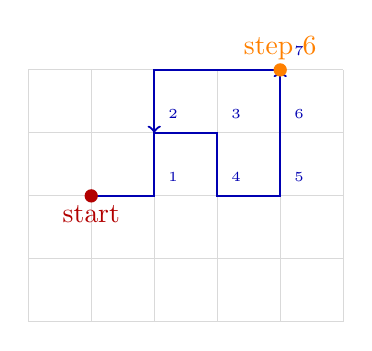
\begin{tikzpicture}[scale=0.8]
  \draw[gray!30,thin] (0,0) grid[step=1] (5,4);
  \draw[blue!70!black,thick,->] (1,2)--(2,2)--(2,3)--(3,3)--(3,2)--(4,2)--(4,3)--(4,4);
  \draw[blue!70!black,thick,->] (4,4)--(3,4)--(2,4)--(2,3);
  \fill[red!70!black] (1,2) circle (3pt) node[below] {start};
  \fill[orange] (4,4) circle (3pt) node[above] {step 6};
  \foreach \x/\y/\s in {2/2/1, 2/3/2, 3/3/3, 3/2/4, 4/2/5, 4/3/6, 4/4/7} {
    \node[font=\tiny,blue!70!black] at (\x+0.3,\y+0.3) {\s};
  }
\end{tikzpicture}
\caption{Random walk on a grid: at each step, move to a uniformly random neighboring vertex.}
\label{fig:random_walk}
\end{figure}


\subsection{Pseudocode}

\subsubsection{Simple 2D Random Walk (Continuous)}
\begin{algorithm}
\caption{2D Random Walk}\label{alg:random_walk_2d}
\begin{algorithmic}
\Function{RandomWalk2D}{start\_point, num\_steps, step\_size}
    \State $current \gets start\_point$
    \State $path \gets [current]$

    \For{$i \text{ in range}(num\_steps)$}
        \Comment{1. Choose random direction}
        \State $\theta \gets \text{random.uniform}(0, 2\pi)$

        \Comment{2. Update position}
        \State $dx \gets step\_size \cdot \cos(\theta)$
        \State $dy \gets step\_size \cdot \sin(\theta)$
        \State $current \gets \text{Point}(current.x + dx, current.y + dy)$
        \State $path.\text{append}(current)$
    \EndFor

    \Return $path$
\EndFunction
\end{algorithmic}
\end{algorithm}

\subsubsection{Random Walk on a Mesh}
\begin{algorithm}
\caption{Random Walk on a Mesh}\label{alg:mesh_random_walk}
\begin{algorithmic}
\Function{MeshRandomWalk}{mesh, start\_v, num\_steps}
    \State $current\_v \gets start\_v$
    \State $visited\_v \gets [current\_v]$

    \For{$i \text{ in range}(num\_steps)$}
        \State $neighbors \gets \text{mesh.GetNeighbors}(current\_v)$
        \Comment{1. Choose a random neighbor}
        \State $current\_v \gets \text{random.choice}(neighbors)$
        \State $visited\_v.\text{append}(current\_v)$
    \EndFor

    \Return $visited\_v$
\EndFunction
\end{algorithmic}
\end{algorithm}

\subsection{Parameter Selection}
\begin{itemize}
    \item \textbf{Step Size}: Constant step size vs.\ variable (Gaussian) step size.
    \item \textbf{Connectivity}: On a grid, 4-connectivity (von Neumann) vs.\ 8-connectivity (Moore).
    \item \textbf{Weights}: In weighted random walks, the probability of a step is proportional to some value (e.g., $e^{-\Delta E / kT}$).
\end{itemize}

\subsection{Complexity}
\begin{itemize}
    \item \textbf{Time Complexity}: $O(n)$ where $n$ is the number of steps.
    \item \textbf{Space Complexity}: $O(n)$ to store the full path, or $O(1)$ if only the final position is needed.
\end{itemize}

\subsection{Usages}
\begin{itemize}
    \item \textbf{Monte Carlo Simulation}: Estimating areas or volumes of complex shapes (Hit-or-Miss Monte Carlo).
    \item \textbf{Mesh Analysis}: Using random walks to calculate ``closeness'' between vertices or to partition meshes.
    \item \textbf{Generative Art}: Creating organic, branching patterns (e.g., Diffusion-Limited Aggregation).
    \item \textbf{Network Science}: Identifying communities in a graph or calculating PageRank.
    \item \textbf{Finance}: Modeling stock price movements (Geometric Brownian Motion).
    \item \textbf{Physics}: Simulating the movement of gas particles or the propagation of heat.
\end{itemize}

\subsection{Testing Methods and Edge Cases}
\begin{itemize}
    \item \textbf{Mean Position}: Verify that after many trials, the average final position of an isotropic walk is the starting point.
    \item \textbf{Scaling Law}: Verify that the distance from the start grows as $\sqrt{n}$ on average.
    \item \textbf{Boundaries}: Test how the walk behaves when it hits a wall (e.g., reflection vs.\ absorption).
    \item \textbf{Mesh Boundaries}: Ensure the walker doesn't ``fall off'' the edge of an open mesh.
    \item \textbf{Looping}: Observe how often the walker visits the same vertex in 2D vs.\ 3D.
\end{itemize}

\subsection{References}
\begin{itemize}
    \item Pearson, K. (1905). ``The Problem of the Random Walk''. Nature.
    \item Polya, G. (1921). ``\"Uber eine Aufgabe der Wahrscheinlichkeitsrechnung betreffend die Irrfahrt im Stra{\ss}ennetz''. Mathematische Annalen.
    \item Spitzer, F. (1976). ``Principles of Random Walk''. Springer.
    \item Wikipedia: Random walk
\end{itemize}


\section{Self-Avoiding Walk}
\label{sec:self_avoiding_walk}

\subsection{Overview}
A \index{self-avoiding walk}self-avoiding walk (SAW) is a sequence of moves on a lattice (such as a 2D or 3D grid) that does not visit the same point more than once. Unlike a simple random walk, which can cross its own path, a SAW must satisfy the constraint of self-exclusion. This exclusion makes SAWs significantly more difficult to analyze and simulate, as the ``future'' path depends on the entire ``history'' of the walk~\cite{madras1996}.

\subsection{Definitions}
\begin{definition}[Lattice]\label{def:saw_lattice}
A regular grid of points (e.g., square, hexagonal, cubic). The lattice determines the set of allowed moves at each step.
\end{definition}

\begin{definition}[Length ($n$)]\label{def:saw_length}
The number of steps in the walk. The walk consists of $n + 1$ vertices and $n$ edges.
\end{definition}

\begin{definition}[Connective Constant ($\mu$)]\label{def:connective_constant}
A lattice-specific constant describing the exponential growth rate of the number $c_n$ of possible SAWs of length $n$: $c_n \sim A \mu^n n^{\gamma - 1}$ as $n \to \infty$, where $\gamma$ is a universal critical exponent depending only on the dimension~\cite{madras1996}.
\end{definition}

\begin{definition}[End-to-End Distance]\label{def:end_to_end_distance}
The Euclidean distance between the starting point and the final point of the walk. For a SAW of length $n$, the mean end-to-end distance scales as $\langle R^2 \rangle \sim n^{2\nu}$ where $\nu$ is the \index{Flory exponent}Flory exponent ($\nu \approx 3/4$ in $d=2$)~\cite{flory1953}.
\end{definition}

\subsection{Theory}
The number of simple random walks of length $n$ on a $d$-dimensional lattice is exactly $(2d)^n$. For SAWs, there is no simple formula. The number of SAWs $c_n$ is known to behave as $c_n \sim A \mu^n n^{\gamma-1}$, where $\mu$ depends on the lattice and $\gamma$ is a ``universal'' exponent that depends only on the dimension~\cite{madras1996}.

Generating SAWs is a challenge due to \textbf{attrition}: if you build a walk step-by-step randomly, you often get ``trapped'' where all neighboring points have already been visited. This leads to several simulation strategies:
\begin{enumerate}
    \item \textbf{Simple Sampling}: Generate random walks and discard them if they intersect themselves. (Extremely inefficient for large $n$).
    \item \textbf{Pivot Algorithm}: Start with a valid SAW and apply a symmetry operation (rotation or reflection) to a portion of the walk. If the result is still self-avoiding, accept it. This is the most efficient known method for generating long SAWs.
    \item \textbf{Rosenbluth Method}: A weighted sampling method that avoids immediate self-intersections but suffers from diminishing weights.
\end{enumerate}

\begin{theorem}[Connective Constant Bounds]\label{thm:connective_constant}
For the square lattice $\mathbb{Z}^2$, the connective constant satisfies $\mu \le 2 + \sqrt{2} \approx 3.414$ (the Madras--Slade bound). Exact values are known only for self-avoiding walks on certain special lattices. For the hexagonal lattice, $\mu = \sqrt{2 + \sqrt{2}} \approx 1.848$~\cite{madras1996}.
\end{theorem}

\begin{proof}
The upper bound $\mu \le 2 + \sqrt{2}$ is proved using the lace expansion technique, which decomposes the SAW into a random walk plus correction terms that account for self-avoidance. The key identity relates the two-point function of the SAW to that of the simple random walk through a renormalization argument. For the hexagonal lattice, the exact value follows from a combinatorial argument using the correspondence between SAWs and the zero-field Ising model at the critical temperature~\cite{madras1996}.
\end{proof}

\begin{example}[Number of SAWs on $\mathbb{Z}^2$ for Small $n$]\label{ex:saw_counts}
The exact counts $c_n$ of self-avoiding walks on the square lattice starting from the origin:
\begin{center}
\begin{tabular}{cc}
\toprule
$n$ & $c_n$ \\
\midrule
1 & 4 \\
2 & 12 \\
3 & 36 \\
4 & 100 \\
5 & 284 \\
6 & 780 \\
\bottomrule
\end{tabular}
\end{center}
From these values, one can estimate $\mu \approx c_{n+1}/c_n \to \mu \approx 2.64$ as $n$ grows, converging to the true value $\mu \approx 2.638$.
\end{example}

\subsection{Pseudocode}

\subsubsection{Simple Recursive SAW Generator}
\begin{algorithm}
\caption{Generate Self-Avoiding Walk (Recursive)}\label{alg:generate_saw}
\begin{algorithmic}
\Function{GenerateSAW}{path, n, lattice}
    \If{$\text{len}(path) = n$}
        \Return $path$
    \EndIf

    \State $current \gets path[-1]$
    \State $neighbors \gets \text{lattice.GetNeighbors}(current)$

    \Comment{Shuffle neighbors to explore randomly}
    \State $\text{random.shuffle}(neighbors)$

    \ForAll{$neighbor \in neighbors$}
        \If{$neighbor \notin path$}
            \Comment{1. Recursive attempt}
            \State $result \gets \text{GenerateSAW}(path + [neighbor], n, lattice)$
            \If{$result \neq \text{None}$}
                \Return $result$
            \EndIf
        \EndIf
    \EndFor

    \Comment{2. Dead end (Backtrack)}
    \Return $\text{None}$
\EndFunction
\end{algorithmic}
\end{algorithm}
Note that \Cref{alg:generate_saw} uses exhaustive backtracking. For large $n$, the \textbf{pivot algorithm} is far more efficient, achieving near-$O(n)$ amortized cost per sample~\cite{madras1996}.

\subsection{Parameter Selection}
\begin{itemize}
    \item \textbf{Lattice Type}: Square (4 neighbors) and Hexagonal (3 neighbors) are common in 2D.
    \item \textbf{Algorithm}: Use the \textbf{Pivot Algorithm} for generating very long SAWs (thousands of steps) as it is much faster than simple recursion or sampling.
\end{itemize}

\subsection{Complexity}
\begin{itemize}
    \item \textbf{Simple Recursion}: $O(\mu^n)$ in the worst case, as it is an exhaustive search.
    \item \textbf{Pivot Algorithm}: $O(n)$ or even $O(n^{0.5})$ per successful update, making it feasible for $n \approx 10^6$.
    \item \textbf{Space Complexity}: $O(n)$ to store the coordinates of the walk.
\end{itemize}

\subsection{Usages}
\begin{itemize}
    \item \textbf{Polymer Physics}: SAWs are the standard model for ``linear polymers'' in a good solvent, where the exclusion principle represents the ``excluded volume'' of atoms~\cite{flory1953}.
    \item \textbf{Proteins}: Modeling the backbone of a protein during folding.
    \item \textbf{Network Science}: Analyzing paths in social or communication networks where nodes shouldn't be repeated.
    \item \textbf{Material Science}: Studying the distribution of chains in a porous medium.
    \item \textbf{Combinatorics}: A fundamental problem in counting and probability.
\end{itemize}

\subsection{Testing Methods and Edge Cases}
\begin{itemize}
    \item \textbf{No Intersections}: Verify that all points in the generated path are unique.
    \item \textbf{Connectivity}: Ensure each point in the path is a valid neighbor of the previous point on the lattice.
    \item \textbf{Connective Constant}: Verify that for small $n$, the number of generated SAWs matches known exact counts (\cref{ex:saw_counts}).
    \item \textbf{Lattice Boundaries}: If the walk is confined to a box, ensure it handles the boundaries correctly.
    \item \textbf{Trap Detection}: Verify the algorithm correctly backtracks or terminates when the walker is surrounded by visited points.
\end{itemize}

\subsection{References}
\begin{itemize}
    \item Madras, N., \& Slade, G. (1996). ``The Self-Avoiding Walk''. Birkh\"{a}user.
    \item Flory, P. J. (1953). ``Principles of Polymer Chemistry''. Cornell University Press.
    \item Kennedy, T. (2002). ``A faster implementation of the pivot algorithm for self-avoiding walks''. Journal of Statistical Physics.
    \item Wikipedia: Self-avoiding walk
\end{itemize}
